\documentclass{article}
\usepackage[utf8]{inputenc}

\usepackage{graphicx}
\usepackage[T1]{fontenc}
\usepackage{graphicx}
\usepackage{grffile}
\usepackage{longtable}
\usepackage{wrapfig}
\usepackage{rotating}
\usepackage[normalem]{ulem}
\usepackage{amsmath}
\usepackage{textcomp}
\usepackage{amssymb}
\usepackage{capt-of}
\usepackage{hyperref}
\usepackage[margin=2cm]{geometry}
\usepackage{xfrac}
\usepackage{float}

\title{TREBALL PRÀCTIC 2}
\author{Eric Valls, Victor Martin, Dean Zhu}
\date{December 2017}

\begin{document}

\maketitle
\section{P1}
\label{sec:orgc9ba521}
\subsection{Metode del trapezi i quadratura de Newton}
\label{sec:org8b1c0b6}
\subsubsection{Valors obtinguts:}
\label{sec:org29610ac}
\begin{center}
\begin{tabular}{lrrrrrr}
Subintervals & 4 & 8 & 16 & 32 & 64 & 128\\
\hline
Quadratura de Simpson & 0.5811321 & 0.3350465 & 0.1059936 & 0.3529160 & 0.3162173 & 0.3159170\\
Metode del Trapezi & 1.1027294 & 0.7115314 & 0.4291677 & 0.1867871 & 0.3113838 & 0.3150090\\
\end{tabular}
\end{center}

\begin{center}
\begin{tabular}{lrrrrrr}
Subintervals & 256 & 512 & 1024 & 2048 & 4096 & 8192\\
\hline
Quadratura de Simpson & 0.3159050 & 0.3159043 & 0.3159043 & 0.3159043 & 0.3159043 & 0.3159043\\
Metode del Trapezi & 0.3156900 & 0.3158513 & 0.3158911 & 0.3159010 & 0.3159035 & 0.3159041\\
\end{tabular}
\end{center}

\begin{figure}[htbp]
\centering
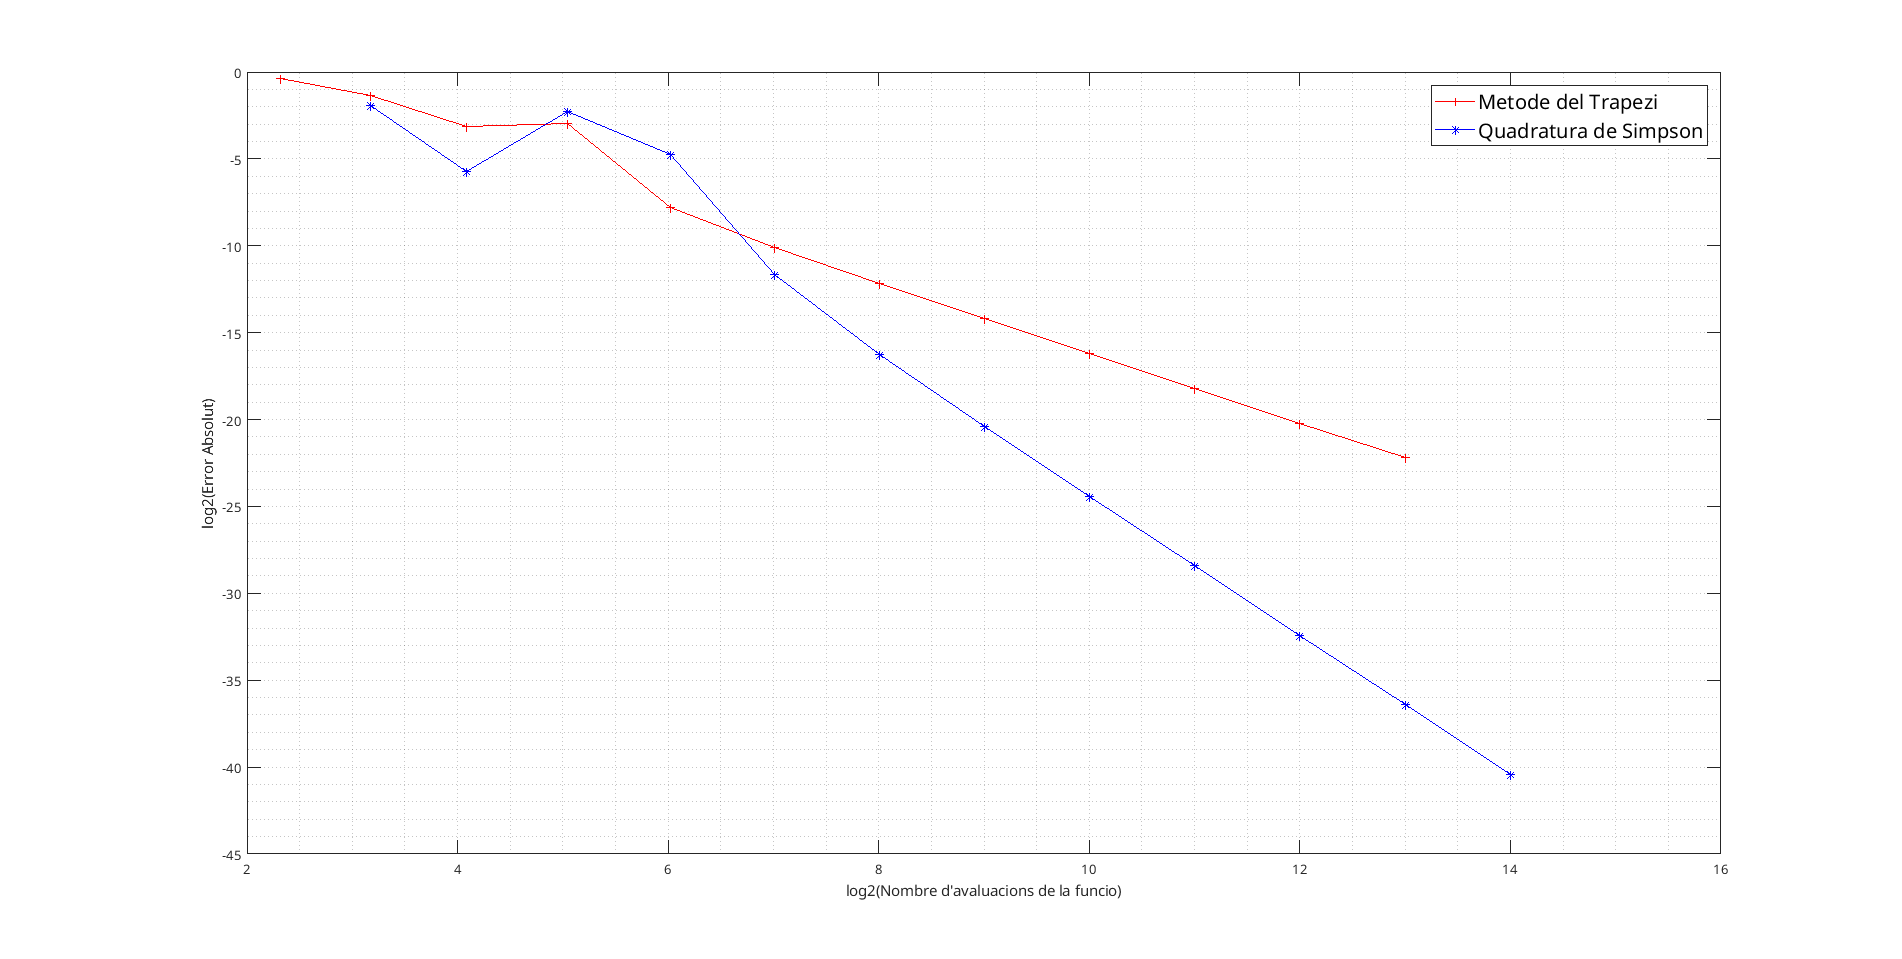
\includegraphics[width=.9\linewidth]{./TrapezivsSimpson.png}
\caption{\label{fig:orged97759}
Convergencia de les quadratures}
\end{figure}

Observem que ambdos metodes convergeixen correctement, el metode del trapezi te una convergencia quadratica i la quadratura de Simpson una convergencia proporcional a m\(^{\text{4}}\).
\subsubsection{Cota de l'error}
\label{sec:orga7a8e4b}
\begin{enumerate}
\item Quadratura composta del trapezi
\label{sec:org48270c9}

Sabem que la quadratura composta del trapezi comet un error de: 
\[
 E_m = -\frac{(b-a)^3}{12m^2}f^{''}(\mu) =  -\frac{2}{3m^2}f^{''}(\mu) 
\]
\[
 f^{''} = 4e^{2x}cos(e^{2x}) - 4e^{4x}sin(e^{2x})
\]
La segona derivada assoleix un maxim valor absolut en el punt x = 2, i \(f^{''}(2) \approx 11000\). Per tant:
\[
\lvert E_m \rvert \leq \bigg\lvert \frac{2\cdot11000}{3} \cdot m^{-2} \bigg\rvert
\] 
Llavors si volem un error menor a 10\(^{\text{-6}}\):
\[
85000 \approx \sqrt{\frac{2\cdot11000}{10^{-6} * 3}} \geq m
\]

Ens dona una fita clarament massa alta (amb 8192 intervals, la quadratura composta del trapezi nomes comet un error de \(2\cdot10^{-7}\)).

\begin{figure}[htbp]
\centering
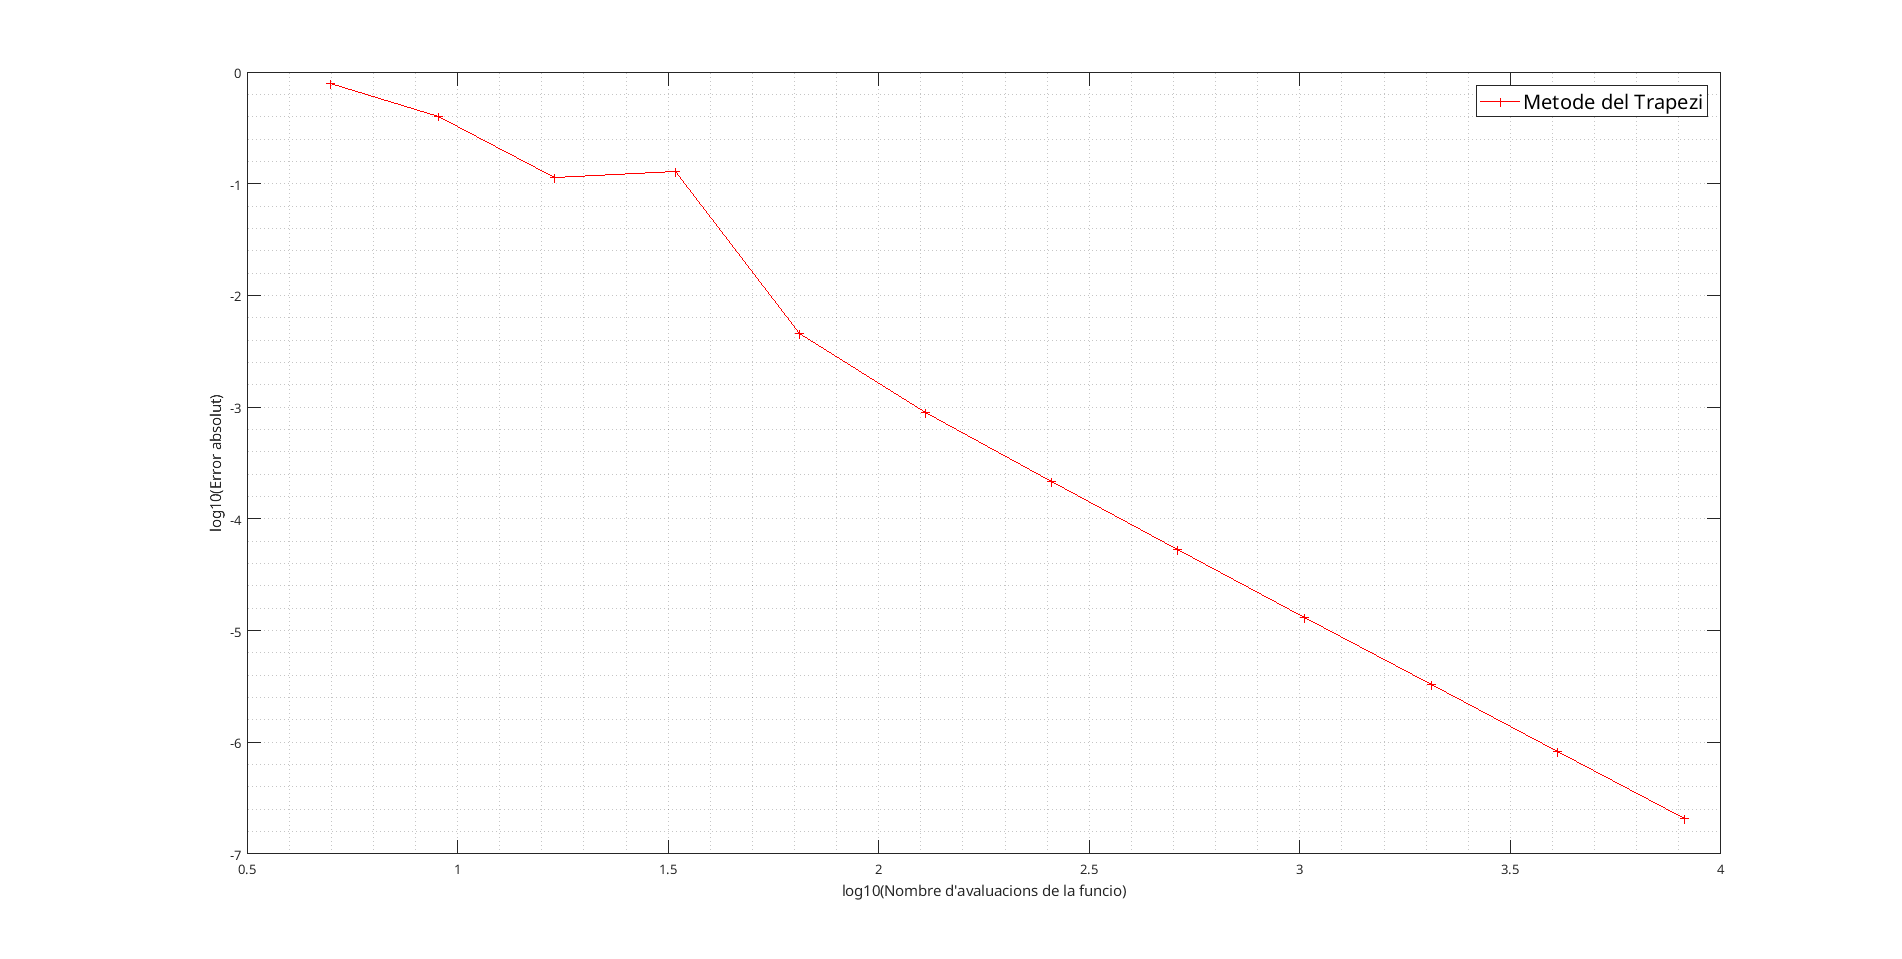
\includegraphics[width=.9\linewidth]{./Trapezilog10.png}
\caption{Logaritme en base 10 del error del metode del Trapezi}
\end{figure}

Ara be, si ens fixem en la grafica del error, sembla que el metode cometra un error absolut de 10\(^{\text{-6}}\) quan s'avalua amb 10\(^{\text{3.6}}\) \(\approx 4000\) cops.
Si suposem que la funcio del error es prou monotonament decreixent podem fer una cerca dicotomica i obtenim que el nombre de intervals necessaris son 3722.
Si avaluem aquestes fites, veiem que la quadratura retorna els valors seguents
\begin{center}
\begin{tabular}{rrll}
Intervals & Valor & Error Absolut & Error Relatiu\\
\hline
3722 & 0.3159032851 & 9,99959 \(\cdot\) 10\(^{\text{-7}}\) & 3.16538 \(\cdot\) 10\(^{\text{-6}}\)\\
4000 & 0.3159034192 & 8.65787 \(\cdot\) 10\(^{\text{-7}}\) & 2.74066 \(\cdot\) 10\(^{\text{-6}}\)\\
85000 & 0.3159402831 & 1.91722 \(\cdot\) 10\(^{\text{-9}}\) & 6.06899 \(\cdot\) 10\(^{\text{-9}}\)\\
\end{tabular}
\end{center}
Sembla ser que la cota real esta mes propera a l'aproximacio obtinguda mirant la grafica. 

\item Quadratura composta de Simpson
\label{sec:orga76fc2e}

Prenent un altre cop la fita del error en funcio de m: 

\[
\lvert E_m \rvert = \bigg\lvert \frac{(b-a)^5}{2880m^4}f^{4)}(\mu) \bigg\rvert
\]
\[
f^{4)}(\mu) = -112e^{4x}sin(e^{2x})+16e^{8x}sin(e^{2x})+16e^{2x}cos(e^{2x})-96e^{6x}cos(e^{2x})
\]
i assoleix un maxim en valor absolut en el punt x = 2, on val 1.26\(\cdot 10^8\). Per tant
\[
\lvert E_m \rvert \leq \bigg\lvert \frac{2^5\cdot 1.26 \cdot 10^8}{2880\cdot m^4} \bigg\rvert
\] 
Llavors si volem un error menor a 10\(^{\text{-6}}\):
\[
 m \leq \sqrt[\leftroot{-3}\uproot{3}4]{\bigg\lvert \frac{1^5\cdot 1.26 \cdot 10^8}{2880 \cdot 10^-66} \bigg\rvert} \approx 10^{12} 
\]
En aquest cas obtenim una cota massa gran per poderla avaluar en una maquina. En qualsevol cas sabem que aquesta cota es massa alta ja que quan m = 512 la quadratura composta de Simpson nomes comet un error de 10\(^{\text{-6}}\).

\begin{figure}[htbp]
\centering
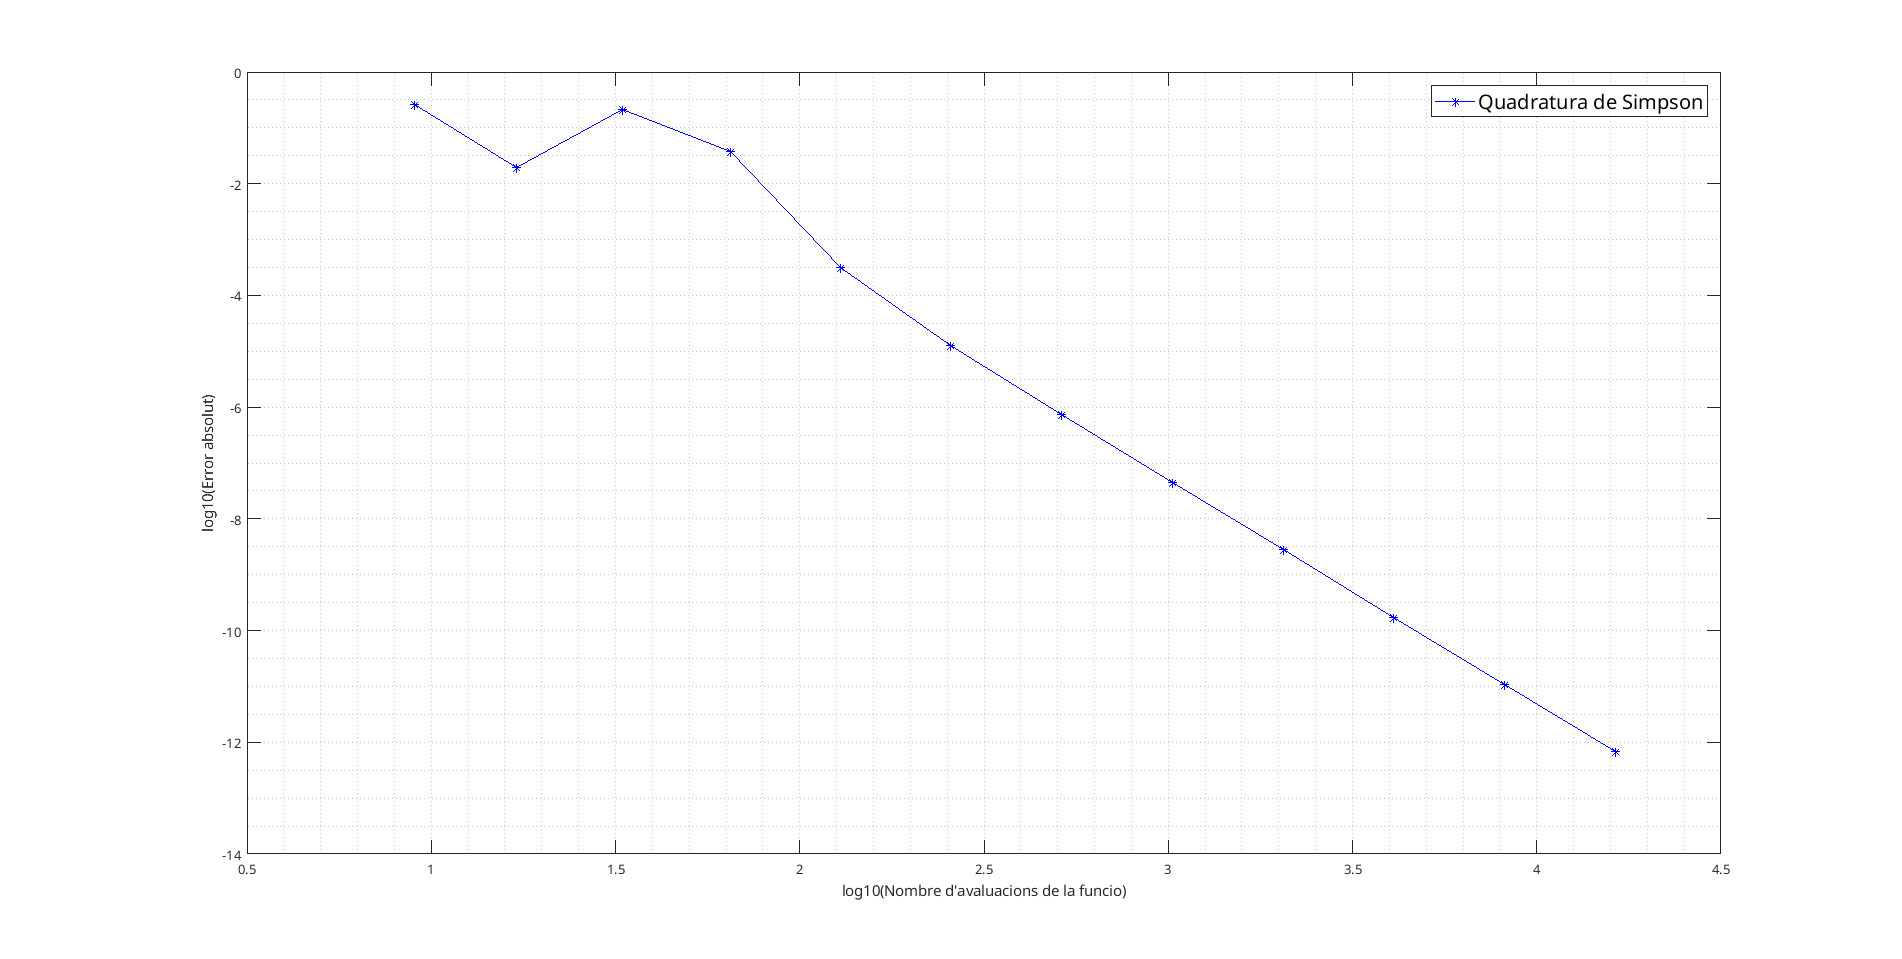
\includegraphics[width=.9\linewidth]{./Simpsonlog10.png}
\caption{Logaritme en base 10 del error de la quadratura de Simpson}
\end{figure}

Si ens fixem en la grafica podem observar que una fita raonable es 10\(^{\text{2,8}}\) \(\approx 630\). Com la grafica es en funcio de les avaluacions prenem la meitat.
Si suposem un altre cop que l'error es prou monoton podem fer una cerca dicotomica i ara obtenim que el nombre d'intervals necessaris son 237.
Si avaluem les fites obtenim:
\begin{center}
\begin{tabular}{rrll}
Intervals & Valor & Error Absolut & Error Relatiu\\
\hline
237 & 0.31590528 & 9.986834 \(\cdot\) 10\(^{\text{-7}}\) & 3.161348 \(\cdot\) 10\(^{\text{-6}}\)\\
315 & 0.31590460 & 3.154840 \(\cdot\) 10\(^{\text{-7}}\) & 9.986699 \(\cdot\) 10\(^{\text{-7}}\)\\
\end{tabular}
\end{center}
\end{enumerate}
\subsection{Quadratura de Simpson Adaptada}
\label{sec:org52b186e}
\subsubsection{Fita del Error}
\label{sec:org5253b07}
Volem veure que la quadratura de Simpson adaptada ens produeix un error fitat (per \(2\epsilon\) en aquest cas). Considerem tots els intervals (x\(_{\text{i}}\), y\(_{\text{i}}\)) tals que retornen el valor de la quadratura sense fer la crida recursiva. Sigui E\(_{\text{i}}\) l'error comes per l'interval i-essim, com tots aquests intervals son disjunts i la seva unio es (0,2) tenim que:
\[ \sum_{i=0}^{r} E_{i} < \sum_{i=0}^{r} (y_i - x_i)*\epsilon = (b-a)*\epsilon = 2\epsilon \]
Per tant l'error esta fitat per \(2\epsilon.\)
\subsubsection{Valors obtinguts}
\label{sec:orgd243ae8}
Cridant a la funcio amb una tolerancia de 10\(^{\text{-3}}\) obtenim 0.3159217 i un error absolut de 6.4188e-04. mentres que la funcio \emph{integral} a matlab ens retorna 0.3159042. En efecte, hem comes un error menor a 2\(\cdot\)10\(^{\text{-3}}\).

Els intervals que utilitzem en aquest cas son (51 punts):

\begin{figure}[htbp]
\centering
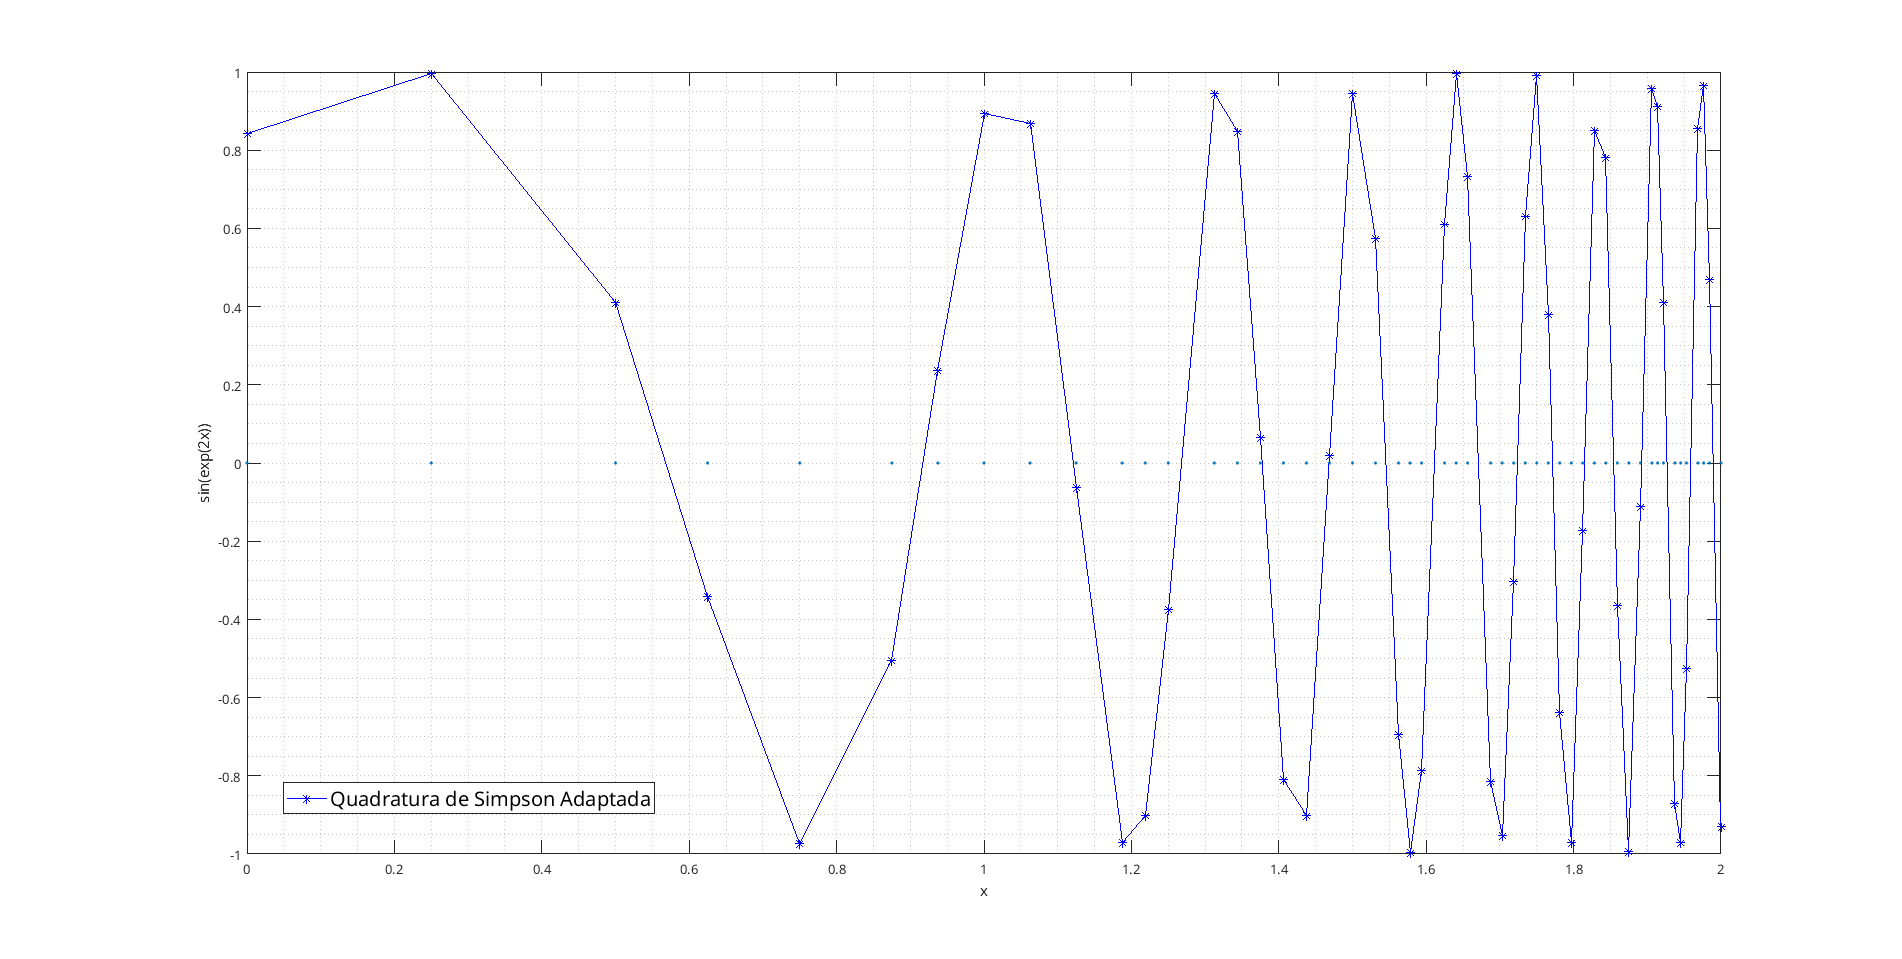
\includegraphics[width=.9\linewidth]{./SimpsonAdaptat.png}
\caption{\label{fig:org1deb30d}
Simpson Adaptat amb tolerancia 10\(^{\text{-3}}\)}
\end{figure}

Si volem una precisio de 10\(^{\text{-6}}\) obtenim com a resposta 0.3159041 i utilitzem 258 punts:

\begin{figure}[H]
\centering
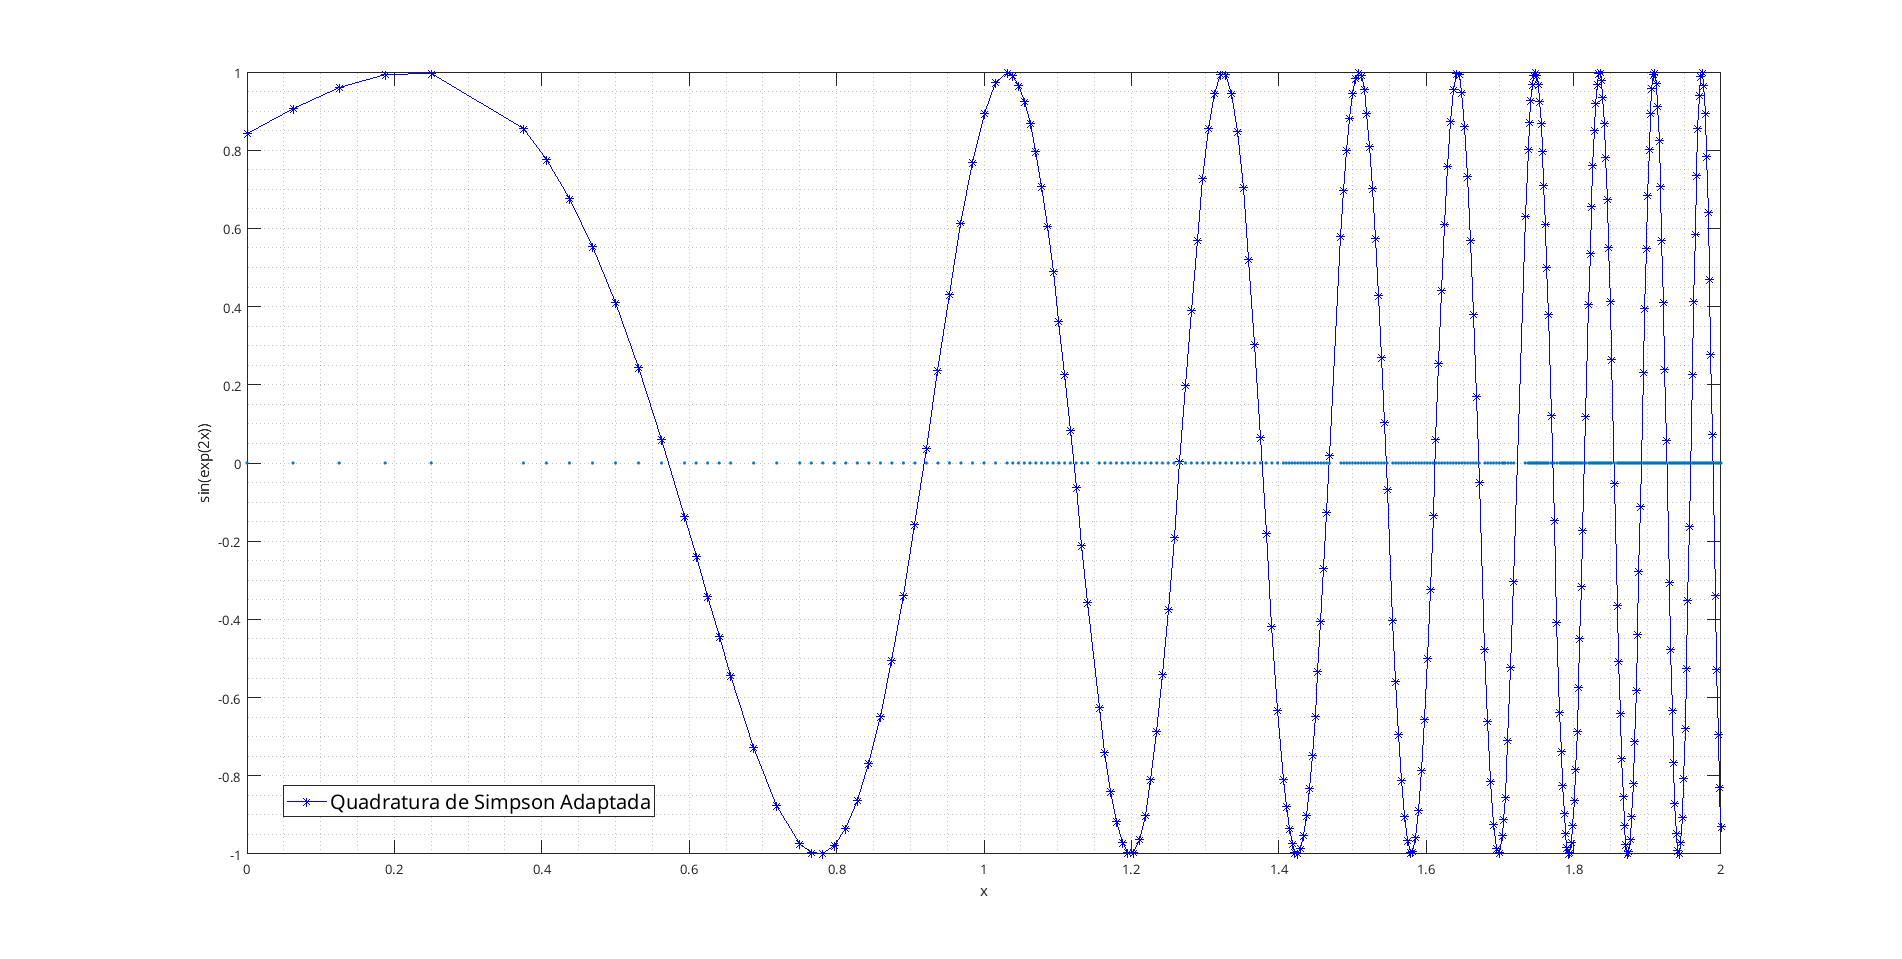
\includegraphics[width=.9\linewidth]{./SimpsonAdaptat2.png}
\caption{\label{fig:org58465fd}
Simpson Adaptat amb tolerancia 10\(^{\text{-6}}\)}
\end{figure}

Donat que la figura oscil.la molt mes a la esquerre, si utilitzem la quadratura de simpson amb intervals uniformes utilitzem molts mes punts dels que necessitem, ja que a l'interval [0,1] no calen masses punts per poder aproximar el valor de l'integral. La quadratura de Simpson adaptada ens permet aproximar l'integral sense fer servir punts inutils. De fet quan volem una precisio de 10\(^{\text{-6}}\) nomes 36 punts es troben a l'interval [0,1]
\newpage
\section{Problema 2}

\subsection{a}

Per trobar la mínima \emph{m} tal que s(b) tingui 4 xifres significatives correctes farem servir dos mètodes diferents:

Mètode 1: Calculem el valor "exacte" (tot i no ser exacte/real ja que també es calcula numèricament, li direm així ja que l'hem calculat amb precisió màquina pràcticament) de s(b) fent servir la funcio \emph{integral} de Matlab que ens dona que s(b) = 21.228219155979843. Fent servir aquest valor, iterarem per \emph{m} fins que l'error per una \emph{m} donada tingui un error relatiu menor a
$5*10^{-5}$. Aquest mètode ens dona que m = 29. A la següent figura podem veure la gràfica de convergència en escala logarítmica.

\begin{center}
\includegraphics[scale=0.25]{ConvergenciaA.jpg}
\end{center}

Podem veure com per a valors petits de \emph{m} la convergència oscil·la bastant. No obstant, a partir de cert valor, la convergència passa a ser d'ordre entre 4 a 5 com esperàvem al estar fent servir la quadratura composta de Simpson.


Mètode 2: Si no tinguéssim el valor real de la integral (per ser massa costós de calcular, per exemple) no podríem fer servir el mètode anterior. Aquest segon mètode consisteix a iterar per \emph{m} fins que l'error relatiu entre \emph{m} i \emph{m-1} sigui més petit que $5*10^{-5}$. 
Aquest mètode ens dona que m = 21.

Conclusió: El primer mètode dona el resultat correcte però òbviament requereix de tenir un valor real de la integral. No obstant, això en general no ho tindrem en general i haurem servir el mètode 2. Sembla que el mètode 2 hagi calculat \emph{m} amb poca precisió ja que ens ha donat 21 enlloc de 29. Ara, si calculem l'error relatiu de la integral amb \emph{m} = 21 ens dóna 6.243341155780989e-05 que s'apropa bastant a les 4 xifres significatives. Per tant, en aquest cas, el mètode 2 ha funcionat bastant bé. Ara, en general, no podem garantir que funcioni bé en general.


Fent servir m = 29, s(t) = 21.227.

\subsection{b}

Ara, donat un s \( \in \) [s(a), s(b)], volem trobar k \( \in \)[a, b] tal que s(k) = s. Sabem que aquest valor existeix perquè s(t) és contínua i podem aplicar el teorema del valor mitjà. 

Trobar aquesta imatge és equivalent a resoldre s(t) = s que és equivalent a resoldre s(t) - s = 0. Sembla raonable utilitzar un dels mètodes per trobar zeros implementats a la pràctia 1, com per exemple, el mètode de newton. A més a més, observem que com s(t) és creixent (al ser no negativa la funcio a integrar), aquesta equació només té una solució i, per tant, si el mètode de newton convergeix, sabrem que convergeix a la única solució. Triem Newton ja que tenim una derivada numèrica i no biseccio perquè convergeix més rapidament.

\subsection{c}

Volem calcular ara l'antiimatge per s = (s(a) + s(b))/2. Per fer això implementem el que hem fet a l'apartat \emph{b} i iterem newton fins que l'error entre resultats successius sigui menor a $5*10^{-5}$.
L'aproximació inicial la trobem representant la gràfica de la funció que podem veure a la imatge següent.


\begin{center}
\includegraphics[scale=0.25]{graficanewton.jpg}
\end{center}

Aquesta gràfica ens confirma el que hem dit anteriorment (existeix una única solució) i observem que 0.8 sembla una aproximació inicial prou bona pel mètode de Newton. Aplicant el mètode de Newton amb aquesta aproximació inicial, obtenim que k = 0.7988492827.

Si no poguéssim dibuixar la gràfica (per un cost massa alt, per exemple) podríem fer unes quantes iteracions del mètode de la bisecció entre \emph{a} i \emph{b} i després, aplicar Newton.


\subsection{d}

Per trobar una distribució equiespaiada de 35 punts sobre la corba, cal que la distància entre punts consecutius sigui (s(b) - s(a))/34 que és 0.62436. Per tant, $t_{i} = antiimatge(a + h*i), 0 \leq i \leq 34 $. Per tant, hem de calcular aquestes 35 antiimatges amb la funció implementada a l'apartat c. 

Executanr el codi i ens dona per als primers 3 punts:

\begin{center}
\begin{tabular}{c c c c}
t & \(\gamma(t).x\) & \(\gamma(t).y\)  & \(\gamma(t).z\) \\
0.0500 & -4.250 & -0.00008345 & 0.0001473 \\
0.3900 & -4.050 & -0.2950 & 0.4985 \\
0.4650 & -3.538 & -0.5233 & 0.7461
\end{tabular}
\end{center}

Si dibuixem els 35 punts junt amb \(\gamma\) i els connectem amb línies obtenim la següent imatge.

\begin{center}
\includegraphics[scale=0.5]{corba.jpg}
\end{center}
 
 
En aquesta es pot observar com efectivament sembla que els punts són equidistants i aproximen bé \(\gamma \).
 
\end{document}
